\documentclass[12pt]{article}
\usepackage{fullpage}
\usepackage{amsmath}
\usepackage{graphicx}
\usepackage{enumerate}
\usepackage{float}
\usepackage{listings}
\usepackage{longtable}
\usepackage[table]{xcolor}
\usepackage{tabularx}
\usepackage{parskip}
\usepackage[round]{natbib}
\restylefloat{figure}
\title{Gamifying the Transcriptome}
\author{Chidube Ezeozue and Joel Brooks}

\begin{document}
\bibliographystyle{apalike}
\renewcommand\refname{Bibliography}
\maketitle

\begin{abstract}

\end{abstract}

\section{Background}
Alternative splicing is an important functional occurrence in eukaryotes \citep{pan2008deep}. These splicing events allow a single gene to produce multiple mRNA transcripts and thus increases biological complexity, as different isoforms may lead to different proteins or different regulation of the same protein \citep{trapnell2010transcript}. These events are quite common, and evidence suggests they occur in roughly 95\% of multiexonic human genes.

The development of RNA-seq technology has greatly advanced the potential effectiveness of mRNA transcript assembly, but detecting isoforms from the millions of short reads generated by RNA-seq is a computationally daunting problem because the reads are too short to span an entire mRNA transcript. Existing methods are able to asses relative exon abundance for a gene from RNA-seq data with relatively high accuracy \citep{trapnell2009tophat}. However, reconstructing the set of mRNA isoforms that produced those exon abundances is a computationally complex problem. One notable example of such methods, Cufflinks, uses weighted bipartite graphs to find the minimum set of transcripts that explain the set of reads. 

We explored the possibility of humans finding alternative sets of transcripts through a game-like interface. The human solutions were then scored using a formula we developed aided by the ground truth present in simulated read data. Human powered computation has been shown to be of use in biological problems \citep{kawrykow2012phylo, cooper2010predicting}. For example, Phylo allowed humans with no understanding of biology to perform multiple sequence alignment (MSA). Phylo was designed to abstract the underlying biology away by representing nucleotide bases as colored blocks.  The intuition behind such an abstraction is that humans are good at visual pattern recognition problems. Using Phylo, humans were indeed able to outperform state of the art MSA algorithms for certain sequences. We used a similar motivation to explore the idea of humans reconstructing transcript isoforms from relative abundances of exons by conveying the problem in a simple block-based puzzle. This makes it possible for a person with no understanding of computational biology to play and find useful solutions. By abstracting the problem of transcript assembly into a simple puzzle form, we can hopefully use human powered computation to parse RNA-seq data.




\section*{Methods}

\subsection*{Game Overview}
The game is designed to utilized human powered computation to explore transcriptome solutions for certain genes using experimental data from
RNA-seq. Experimental data is first mapped to a genome using a splicing aware read aligner such sat TopHat \citep{trapnell2009tophat}. From these mappings,
relative abidance levels of each exon within a gene are inferred.

When the user first starts the game, they are presented with a puzzle as shown in figure \ref{fig:game screen}. This puzzle represents
the relative abundance of exons within a gene. A player must clear all of the blocks in each column in order to complete the puzzle. Users accomplish this by 
creating and adding transcripts to their list. Single colored blocks represent the abundance of reads mapped just to that exon so they can be removed by any 
transcript that includes that exon. However, blocks with two colors represent the abundance of reads that were mapped to more than one exon. These ``linked"
blocks are removed when \emph{both} exons that the reads mapped to are selected, however, no exons can be selected in between the ``linked" blocks as
we assume a read can only map to more than one exon if those two exons appear contiguously within a transcript. Taking these rules into consideration, the user
tries to build a transcript list that removes all of the blocks in the puzzle and achieves a maximal score. After completion of a puzzle, the user's score for that puzzle is
sent back to the server and stored in the database. The user then has the option to start a new puzzle.
\begin{figure*}[t]

\centering
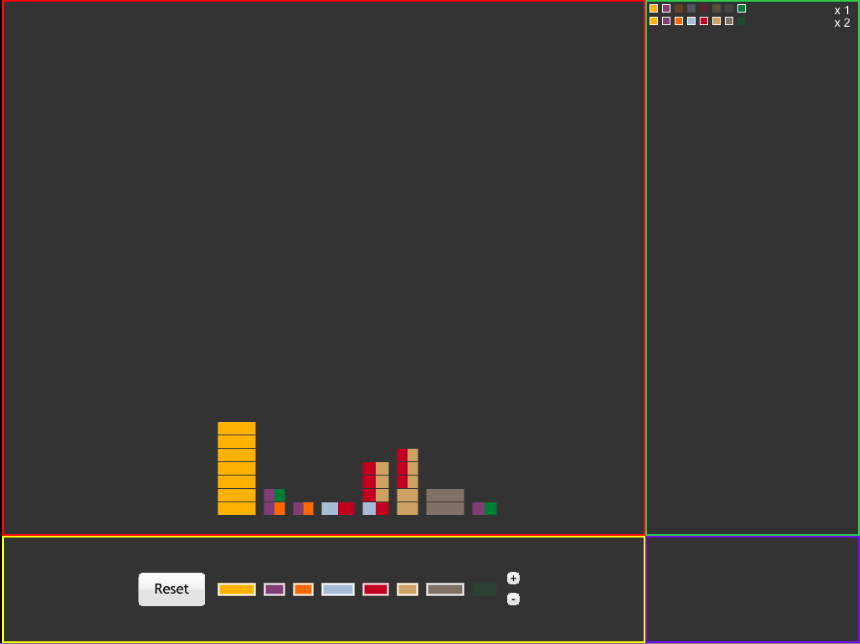
\includegraphics[width=5in]{gamescreen}
\caption{The main game interface}
\label{fig:gamescreen}
\end{figure*}
\subsection*{Data acquisition and preparation}
We simulated short reads using Flux Simulator \cite{sammeth2010flux} running on data from the mouse mm9 genome annotated with the locations of genes, exons and transcripts. To make the problem more tractable, we eliminated all instances of intron-skipping and used only genes with at least 2 transcripts. We, however, ignored the issue of varying transcription starts and represented the data such that all transcripts are assumed to start at the same base in the start exon(s). We simulated over 6 million reads of 75 nucleotides long each and pushed information about read count and mapped exons to the database. Since the simulator created random expression levels for each transcript provided, we only included in the puzzle genes with at least 2 expressed transcripts.

\subsection*{Puzzle selection and construction}

\subsection*{Game implementation}
The game interface is built using the LimeJS HTML5 game framework. This framework provided methods for creating shapes,
animations, and handling user interaction events, allowing us to focus more on developing the core functionality of the game.
Additionally, the fact that the game is implemented in HTML5 and javascript means that it can be played natively in most 
popular browsers, as well as both desktop and mobile hardware.

We also made use of Kenneth Kelly's list of 22 colors of maximum contrast \citep{green2010colour}. This allowed us to assign a unique color each exon
in a particular puzzle that was easily distinguishable from the colors of all the other exons. This allowed us to present genes to 
users in a manner that was both visually appealing and functional.

\subsection*{Solution scoring}
How the user's will approach each puzzle is a function of both the given puzzle and how their solution for that puzzle is scored. Thus, we must have
a proper scoring system in order to influence user's to find accurate lists of transcripts for particular gene. However, as there is no real ``ground truth"
for a list of transcripts for a particular gene, we would like to have a scoring system that is independent of existing transcript annotations. Existing methods
for transcriptome assembly value small lists of unique transcripts, transcripts that include more exons, and transcripts that include more nucleotide bases (citations).
Thus we developed the following scoring metric for scoring transcript list $T$ :
\begin{equation*}
S(T) = d(T) * \sum_{i=1}^{|T|} \log{|T_i|} * \sum_{j = 1}^{|T_i|} \log{n_{ik}}
\end{equation*}
\begin{equation*}
d(T) = \frac{1}{1+e^{\gamma |T|}}
\end{equation*}
where $|T|$ is the number of transcripts in $T$, $|T_i|$ is the number of exons in transcript $T_i$, and $n_{ik}$ is the number of bases in exon $k$ of transcript $i$.
$d$ is a discount factor with parameter $\gamma$ that controls how longer lists of transcripts are devalued. Setting $\gamma = .001$ seemed to achieve the desired
discounting of long transcript lists within the context of the game. Furthermore, the $\log{|T_i|}$ factor ensures that transcripts that only contain one exon will not factor
into the player's score, which is a desirable property given that players often have to add transcripts with one exon in order to finish out a puzzle.

\section*{Results}

\subsection*{Gameplay statistics}

\subsection*{Player solutions}

\section*{Discussion}

We originally planned to have users play puzzles that were generated from real RNA-seq data in addition to the synthetic data generated using Flux Simulator.
We obtained the same experimental RNA-seq data used by Trapnell et al. in the original Cufflinks paper \citep{trapnell2010transcript}. We mapped the reads to 
the mouse genome using TopHat, and were hoping to construct puzzles based on these data in the same manner as we did with the synthetic data. However, due
to time constraints, we felt it was better to focus primarily on the synthetic data, as this allowed us to compare user solutions to a ground truth transcriptome.

Additionally, there are a few aspects of the game implementation that we would like to change before releasing it to the general public. We received mostly
positive feedback from the users that played the game, however, a significant amount of people found the rules of the game to be somewhat confusing. Specifically,
we would like to make the rules regarding ``linked" blocks removal more clear. The confusion was probably due to lack of specific examples of how the ``linked" blocks
work. Thus, adding a tutorial level, gameplay video, or even screenshots that focus on this specific aspect of gameplay would likely help to clear up the confusion.

Another aspect of the game that we'd like to explore is the effect of the within game scoring metric on user solutions. Users are instructed to achieve an optimal score,
and therefore, their solutions should be partially a function of the scoring metric used to evaluate their solutions. However, this relationship could be made more clear by
including a ``high score" that is displayed to the user as they are completing a puzzle. Due to time constraints and limited puzzle coverage, we were unable to include this
feature as part of the game. Furthermore, the scoring metric could be adjusted to change the influence of the different elements involved in scoring a list of transcripts. For example,
one could adjust the scoring metric to make it much more beneficial to include transcripts that have more exons. Ideally, we'd like to explore a number of these possible
metrics, and find the best metric that leads to both good agreement with the ground truth on synthetic data, and still has the ability to find novel transcripts that aren't 
identified by existing computational methods.

\section*{Future Goals}

We'd like to make some of the aforementioned changes to the gameplay interface, and hope to host the game in a location so that it may be played by the general public.
We don't have any current plans to continue analysis, however, we can still store the results in case we come back to this project at a future time. Additionally, the gamification and
visualization of the transcript assembly problem may help to influence similar research projects in the future.

\section*{Comparison with original proposal}

Our main goal from the beginning of the project was to implement the game, and we were able to create a fully functionally final product and test its viability on a select set of users. The main
difference between our original proposal and our final set of accomplishments is the level of detail that the user results were analyzed. We originally wanted to run a pool of algorithms
on the same data that we used to construct the puzzles used in the game, however, we found we weren't able to accomplish this in the time allotted. This became more apparent when we
completed midcourse report, when we further analyzed what we had led to accomplish. However, we feel that the
 algorithmic analysis, while potentially very beneficially, is secondary to the creation and demonstration of the game. Thus, even though we did not achieve all that we had originally set out to
  accomplish, we feel like completed our primary task.

\section*{Commentary on experience}

In General, starting our tasks earlier would have allowed us to better manage time and possibly achieve more of the goals we set out to accomplish in our original project proposal.
There are always unanticipated delays that can be better mitigated by leaving more time than you think you need. For example, data collection was not an issue for us, but
setting up the simulator and analyzing the results was not as trivial as it first seemed. Additionally, there are always unforeseen roadblocks in coding heavy projects, and this project
required a significant amount of programming and development. Identifying these bottlenecks earlier could only help us manage to get by them.

One of the neat things about working on this project is that we have a finished product that we can not only demo, but send out to the general community and have people try it for themselves.
We received quite a bit of feedback from the user base that had played the game, and generally people had positive things to say. We're proud to be able to have the result of the work
that we put in this semester in a packaged form that we can show to people that are not necessarily involved in the computation biology or scientific community.

\section*{Commentary on peer review process}

The reviews were helpful in that they all pointed out that our original timeline was too granular and needed to be broken down. We incorporated an updated timeline in our midcourse
report, which was important as it made us step back and truly analyze how far we had come from when we started the project, and what we had left to do in the time that remained. This
allowed us to better prioritize the items that remained on our agenda, and helped us set a clear path to our project completion. The only other consensus item front he reviews were general
concerns about the playability of the game, however, these felt these points weren't really actionable outside of what we were already aiming to accomplish.

\section*{Division of labor}

Chidube produced the synthetic data with flux simulator, developed and managed the web server and data storage, and performed the post collection data analysis. He also acted as the point
 of first contact with our main project mentor. Joel prepared the experimental RNA-seq data, designed the web browser interface, and was the primary developer of the game functionality and 
 scoring system. Both Chidube and Joel contributed to high level game and project design, as well as writing of the proposals and final report.

\bibliography{frbib}

\end{document}
